Ben Trout

2015-01-16

Building, Brainstorming

\begin{tabular}{|p{5cm}|p{5cm}|}
\hline
Brainstorming&
After our first competition as a team we went through all our weak points and where we could improve our robot. Collectively we decided that there were 6 things that needed to be improved on the robot. The guide tube, ramp, intake, spinner, deflector, and linear slide. We ranked these things from most important to least important and designated each section to a specific person. Matt and Filip redesigned the deflector, Me and Nick were in charge of the intake and linear slide. David was in charge of the redesigned guide tube. Alex was in charge of overlooking all of it and making sure everything went as planned.
\\
\hline
Intake&
Me and Nick first tackled the challenge of the intake. We ended up going with a single axle across the front of the robot to allow more clearance for the big balls and zip tied surgical tubing in a loop fashion around the axle. We also attached a support bar in the front third of the robot to prevent torquing of the robot. We kept the same method of spinning the intake, that is a DC motor with a 1:2 gear ratio to spin it.
\\
\hline
\end{tabular}

\section*{Intake}
Me and Nick were first put in charge or recreating the intake. We had to make it more flexible, allow more clearance, and allow a support channel to be placed near by. Matt researched if Tetrix sold long axles that would span our robot, but to our surprise we actually found a 10in axle. This axle didn’t span our robot though so me and Nick added some 90 degree angles and single channels that allowed us to use this single axle to span the distance. We decided on surgical tubing that would allow us to put on a support beam as the surgical tubing would just bend around the support channel. The only problem with the channel is it took up the space our motor was in. To solve this problem I made the support channel three tall and attached the motor to the support channel and using spacers with long machine screws I got the motor to reach the axle with the same gear ratio as before.

\begin{center}
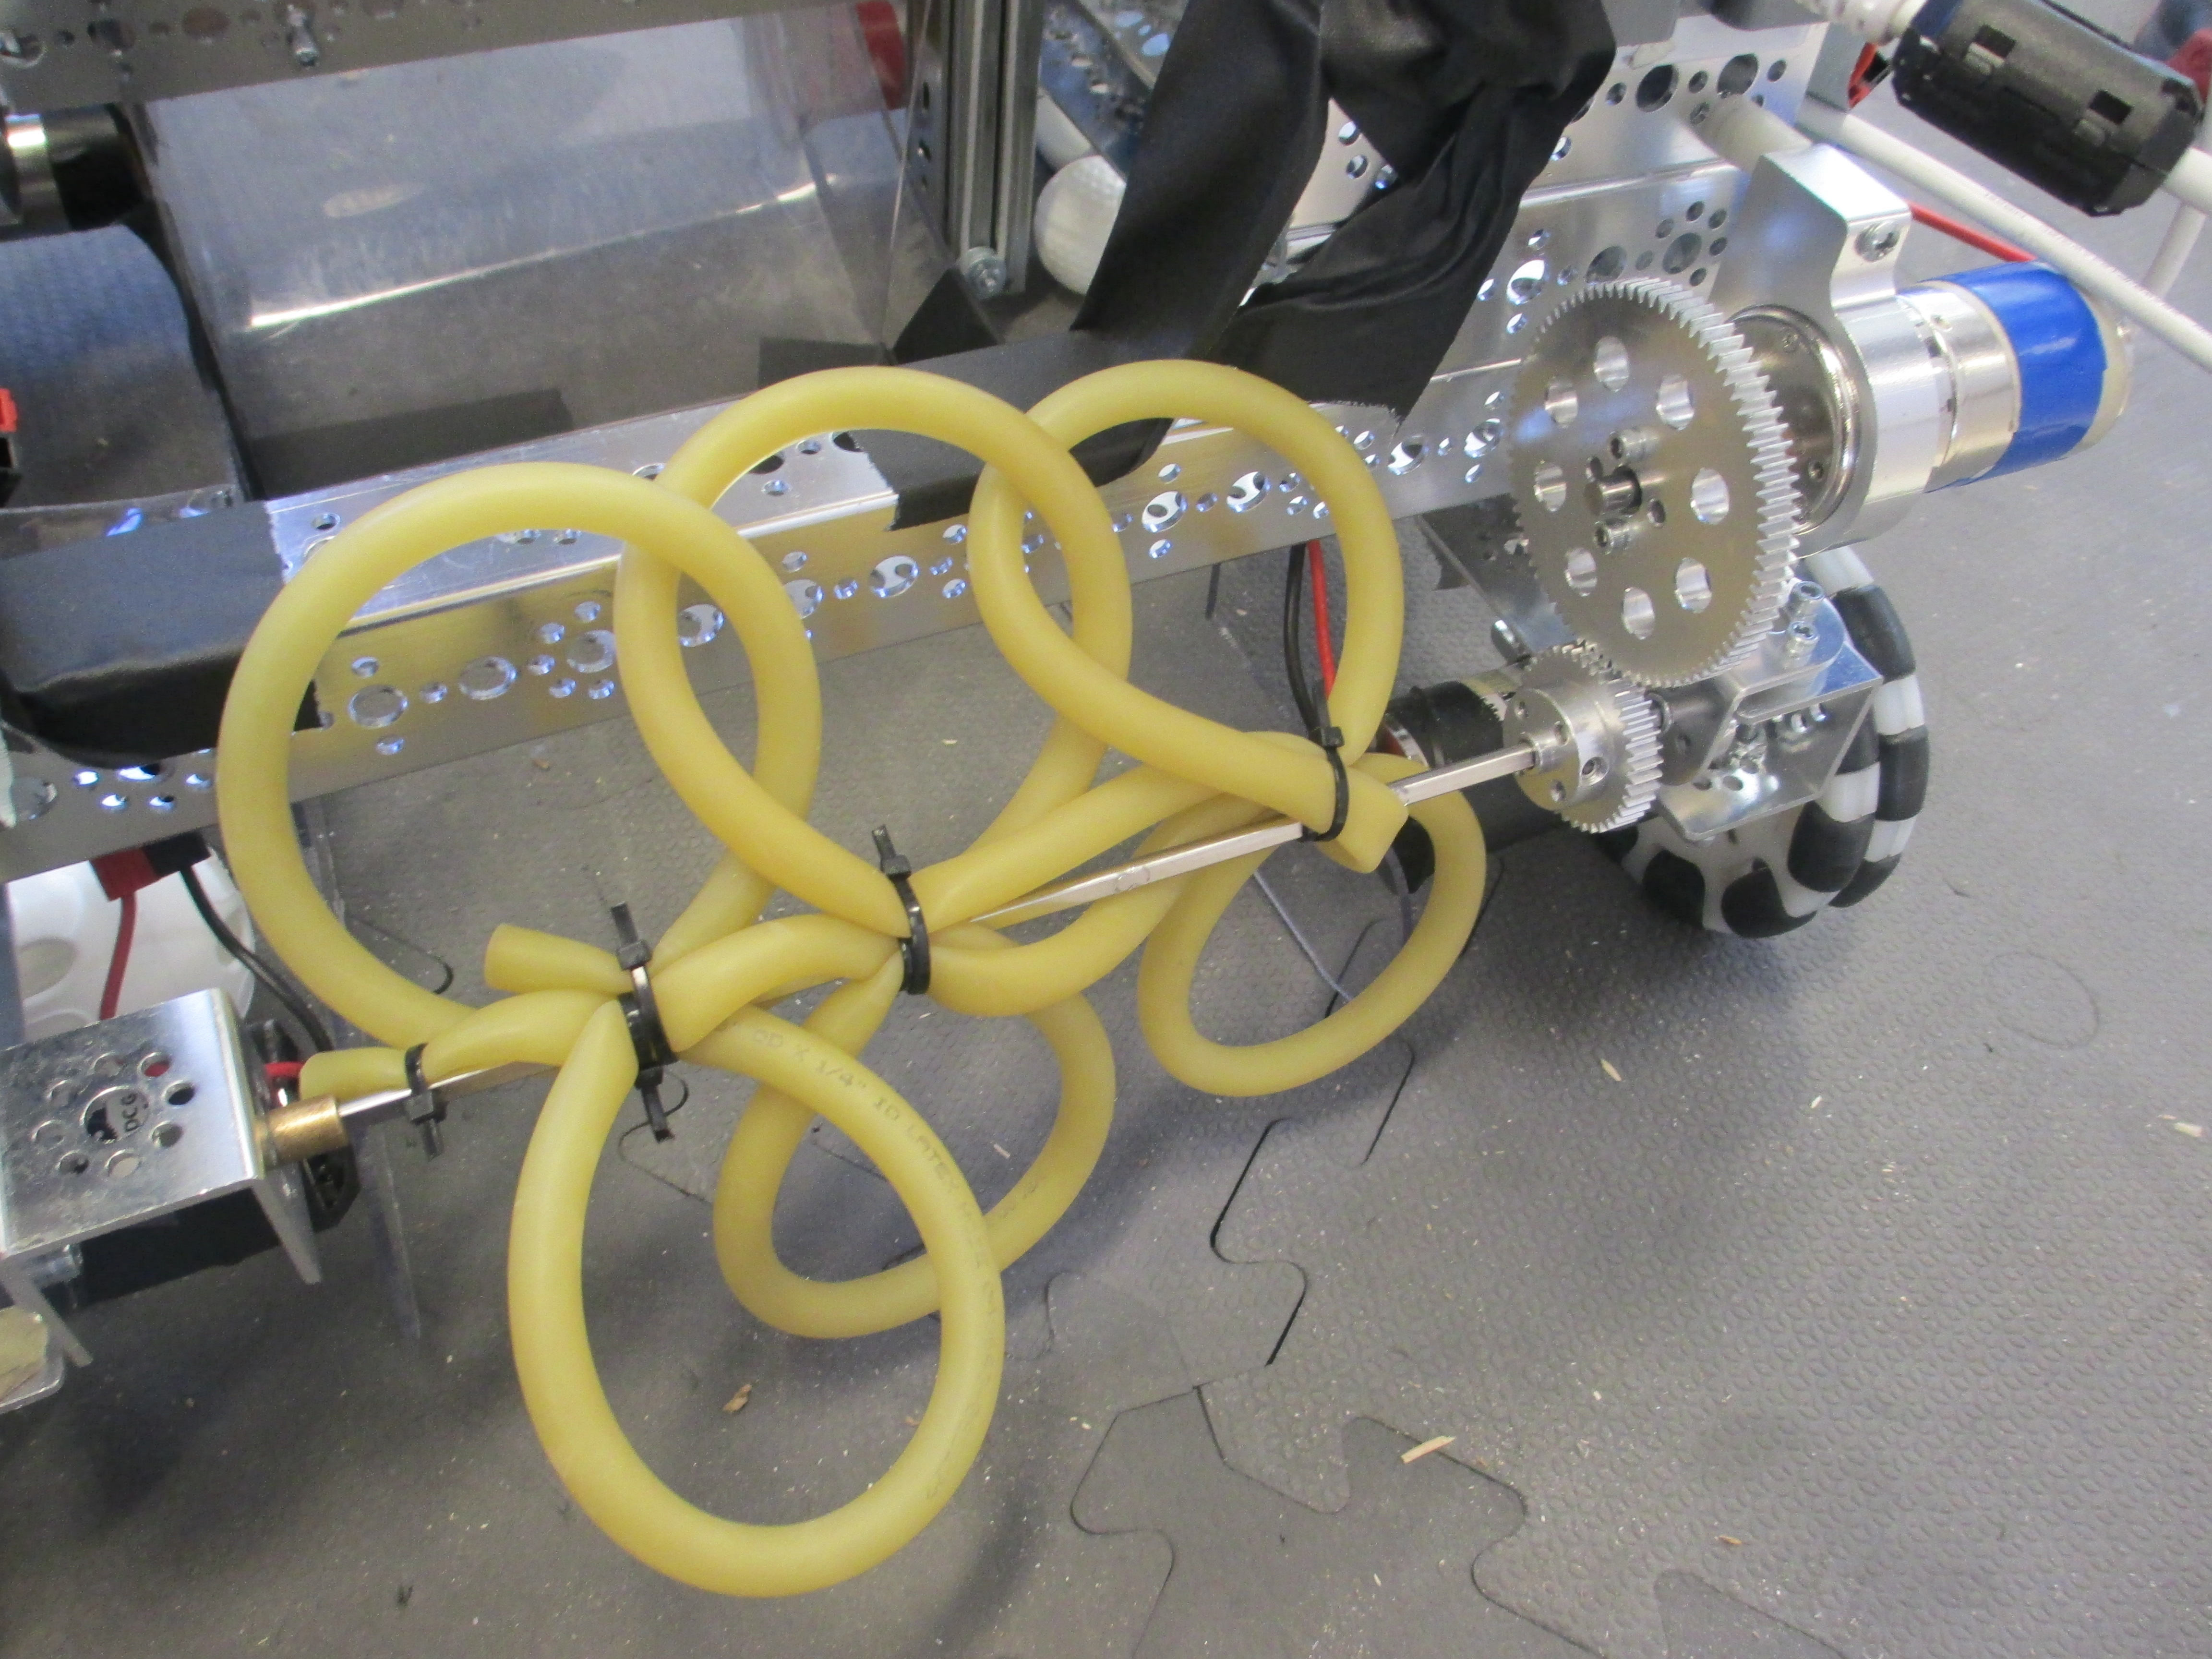
\includegraphics[width=10cm]{./Entries/Images/SurgicalIntake.jpg}
\end{center}

New Intake Design
